\documentclass{article}
\usepackage[utf8]{inputenc}
\usepackage{ctex}
\usepackage{amsfonts}
\usepackage{amsmath}
\usepackage{amssymb}
\usepackage{physics}
\usepackage{graphicx}
\usepackage{geometry}
\geometry{a4paper,left=2cm,right=2cm,top=4cm,bottom=4cm}


\title{地球重力学作业1}
\author{韦淇 \quad 2000012440}
\date{2022年9月6日}

\begin{document}

\maketitle

\section{证明以下等式}
(1)\textbf{\it Proof:}
\begin{align*}
\vec{a}\times(\vec{b}\times\vec{c}) & =  \epsilon_{ijk}a_i(\vec{b}\times\vec{c})_j\hat{e_k} = \epsilon_{kij}a_i\epsilon_{mnj}b_m c_n \hat{e_k}\\
& = \epsilon_{kij}\epsilon_{mnj}a_i b_m c_n \hat{e_k}\\
& = (\delta_{km}\delta_{in} - \delta_{kn}\delta_{im}) a_i b_m c_n \hat{e_k}\\
& = a_i c_i b_k \hat{e_k} - a_i b_i c_k \hat{e_k}\\
& = (\vec{a}\cdot \vec{c})\vec{b} - (\vec{a}\cdot \vec{b})\vec{c}
\end{align*}

(2)\textbf{\it Proof:}
\begin{align*}
    &\curl \grad \phi = \epsilon_{ijk} \phi_{,ji} \hat{e_k} = -\epsilon_{jik} \phi_{,ij} = - \curl \grad \phi \\
    &\Rightarrow \curl \grad \phi = \mathbf{0}
\end{align*}

(3)\textbf{\it Proof:}
\begin{align*}
    &\div (\curl \vec{a}) = \epsilon_{ijk} a_{j,ik} = -\epsilon_{kji} a_{j,ki} = -  \div (\curl \vec{a}) \\
    &\Rightarrow \div (\curl \vec{a}) = 0
\end{align*}

(4)\textbf{\it Proof:}
\begin{align*}
    \grad(UV) &= \hat{e_k}(UV)_{,k} = \hat{e_k}U_{,k}V + \hat{e_k}V_{,k}U \\
    &= V \grad U + U \grad V
\end{align*}

(5)\textbf{\it Proof:}从右往左证
\begin{align*}
    RHS & =  A_i B_{j,i} \hat{e_j} + B_i A_{j,i} \hat{e_j} + \epsilon_{ijk} A_i \epsilon_{mnj} B_{n,m} \hat{e_k} + \epsilon_{ijk} B_i \epsilon_{mnj} A_{n,m} \hat{e_k} \\
    & = A_i B_{j,i} \hat{e_j} + B_i A_{j,i} \hat{e_j} + (\delta_{km}\delta_{in} - \delta_{kn}\delta_{im})A_i B_{n,m} \hat{e_k} \\
    & \quad + (\delta_{km}\delta_{in} - \delta_{kn}\delta_{im})B_i A_{n,m} \hat{e_k}\\
    & = A_i B_{k,i} \hat{e_k} + B_i A_{k,i} \hat{e_k} + A_i B_{i,k} \hat{e_k} - A_i B_{k,i} \hat{e_k} + B_i A_{i,k} \hat{e_k} - B_i A_{k,i} \hat{e_k}\\
    & = A_i B_{i,k} \hat{e_k} + B_i A_{i,k} \hat{e_k} \\
    & = \hat{e_k} \partial_k (A_i B_i) = \grad (\vec{A}\cdot \vec{B})
\end{align*}

(6)\textbf{\it Proof:}从右往左证
\begin{align*}
    RHS & = \hat{e_i} A_{j,ji} - \epsilon_{ijk} \epsilon_{mnj} A_{n,mj} \hat{e_k} \\
    & = \hat{e_i} A_{j,ji} - (\delta_{km}\delta_{in} - \delta_{kn}\delta_{im}) A_{n,mi} \hat{e_k}\\
    & = \hat{e_k} A_{i,ik} - A_{i,ki} \hat{e_k} + A_{k,ii} \hat{e_k} \\
    & = A_{k,ii} \hat{e_k} = \grad^2 A
\end{align*}

\section{证明任意物体的引力场在物体外部为保守力场}
\textbf{\it Proof:} 设$\vec{r}$为场点,$\vec{r'}$为源点,物体区域为V,密度为$\rho(\vec{r'})$。则在物外一点的重力场强度为
\begin{equation*}
    \vec{g}(\vec{r}) = -\int_{V} \frac{\vec{r}-\vec{r'} }{|\vec{r}-\vec{r'}|^3} G\rho(\vec{r'})\mathrm{d^3} \vec{r'}
\end{equation*}
其中$G$为万有引力常数。由于(式中$\grad$是对场点求梯度)
\[
\grad \frac{1}{|\vec{r}-\vec{r'}|} = -\frac{\vec{r}-\vec{r'} }{|\vec{r}-\vec{r'}|^3}
\]
从而
\begin{equation*}
    \vec{g}(\vec{r}) = \int_{V} \grad \frac{1}{|\vec{r}-\vec{r'}|} G\rho(\vec{r'})\mathrm{d^3} \vec{r'} = \grad \int_{V}  \frac{1}{|\vec{r}-\vec{r'}|} G\rho(\vec{r'})\mathrm{d^3} \vec{r'}
\end{equation*}
故重力场$\vec{g}(\vec{r})$ 可写成某一标量场的梯度,所以为保守场。


\section{推导椭球坐标系下的拉普拉斯方程}
椭球坐标与直角坐标的转换关系为
\[
\begin{cases}
x_1 = \sqrt{u^2 + E^2} \sin \theta_r \cos \lambda\\
x_2 = \sqrt{u^2 + E^2} \sin \theta_r \sin \lambda\\
x_3 = u \cos \theta_r
\end{cases}
\]
令空间一点的矢径$\vec{r}$的微分
$$
\mathrm{d}\vec{r} = \frac{\partial \vec{r}}{\partial u}\mathrm{d}u +\frac{\partial \vec{r}}{\partial \theta_r}\mathrm{d}\theta_r +\frac{\partial \vec{r}}{\partial \lambda}\mathrm{d}\lambda \equiv \vec{g}_u \mathrm{d}u + \vec{g}_{\theta_r}\mathrm{d}\theta_r + \vec{g}_{\lambda}\mathrm{d}\lambda,
$$
其中
\begin{align*}
    \vec{g}_u & = \frac{\partial \vec{r}}{\partial u} = \frac{\partial \vec{r}}{\partial x_1}\frac{\partial x_1}{\partial u} + \frac{\partial \vec{r}}{\partial x_2}\frac{\partial x_2}{\partial u} + \frac{\partial \vec{r}}{\partial x_3}\frac{\partial x_3}{\partial u}\\
    & = \hat{e_1} \frac{u}{\sqrt{u^2 + E^2}}\sin\theta_r\cos\lambda + \hat{e_2} \frac{u}{\sqrt{u^2 + E^2}}\sin\theta_r\sin\lambda + \hat{e_3} u \sin\theta_r\\
    \vec{g}_{\theta_r} & = \frac{\partial \vec{r}}{\partial \theta_r} = \frac{\partial \vec{r}}{\partial x_1}\frac{\partial x_1}{\partial \theta_r} + \frac{\partial \vec{r}}{\partial x_2}\frac{\partial x_2}{\partial \theta_r} + \frac{\partial \vec{r}}{\partial x_3}\frac{\partial x_3}{\partial \theta_r}\\
    & = - \hat{e_1} \sqrt{u^2 + E^2} \sin\theta_r\sin\lambda + \hat{e_2} \sqrt{u^2 + E^2}\sin\theta_r\cos\lambda + \hat{e_3} u \sin\theta_r\\
    \vec{g}_{\lambda} & = \frac{\partial \vec{r}}{\partial \lambda} = \frac{\partial \vec{r}}{\partial x_1}\frac{\partial x_1}{\partial \lambda} + \frac{\partial \vec{r}}{\partial x_2}\frac{\partial x_2}{\partial \lambda} + \frac{\partial \vec{r}}{\partial x_3}\frac{\partial x_3}{\partial \lambda}\\
\end{align*}
表示沿椭球坐标系的坐标基矢量,由于
    $$
    \vec{g}_u \cdot \vec{g}_{\theta_r} = \vec{g}_u \cdot \vec{g}_{\lambda} = \vec{g}_{\theta_r} \cdot \vec{g}_{\lambda} = 0
    $$
椭球坐标系为正交坐标系,可以算得$\vec{g}_u, \vec{g}_{\theta_r}, \vec{g}_\lambda$的模分别为
\begin{align*}
    g_u & = \sqrt{\frac{u^2}{u^2+E^2}\sin^2\theta_r + \cos^2 \theta_r} = \frac{\sqrt{u^2 + E^2\cos^2\theta_r}}{\sqrt{u^2+E^2}}\\
    g_{\theta_r} & = \sqrt{(u^2+E^2)\cos^2\theta_r + u^2\sin^2\theta_r} = \sqrt{u^2 + E^2\cos^2\theta_r}\\
    g_\lambda & = \sqrt{u^2+E^2}\sin\theta_r
\end{align*}
用$\hat{u},\hat{\theta_r},\hat{\lambda}$分别表示椭球坐标系下三个方向的单位矢量,则
\[
\mathrm{d}\vec{r} = g_u\mathrm{d}u\hat{u} + g_{\theta_r}\mathrm{d}\theta_r\hat{\theta_r} + g_\lambda \mathrm{d}\lambda \hat{\lambda}
\]

先求梯度在椭球坐标系下的表示,任取一标量场$f$,其全微分为
\[
\mathrm{d}f = \frac{\partial f}{\partial u}\mathrm{d}u + \frac{\partial f}{\partial \theta_r}\mathrm{d}\theta_r + \frac{\partial f}{\partial \lambda}\mathrm{d}\lambda
\]
另一方面
\[
\mathrm{d}f = \grad f \cdot \mathrm{d}\vec{r} = (\grad f)_u g_u \mathrm{d}u + (\grad f)_{\theta_r} g_{\theta_r} \mathrm{d}\theta_r + (\grad f)_\lambda g_\lambda \mathrm{d}\lambda 
\]
比较系数可得
\[
\grad f = \frac{1}{g_u}\frac{\partial f}{\partial u}\hat{u} + \frac{1}{g_{\theta_r}}\frac{\partial f}{\partial \theta_r}\hat{\theta_r} + \frac{1}{g_\lambda}\frac{\partial f}{\partial \lambda}\hat{\lambda}\eqno(1)
\]

再求散度在椭球坐标系下的表示,任取一矢量场$vec{A}$,考察由
\[
g_u\mathrm{d}u\hat{u},\quad g_{\theta_r}\mathrm{d}\theta_r\hat{\theta_r},\quad g_\lambda \mathrm{d}\lambda \hat{\lambda}
\]
三边构成的平行六面体,如图1所示,
\begin{figure}[htbp]
	\centering
	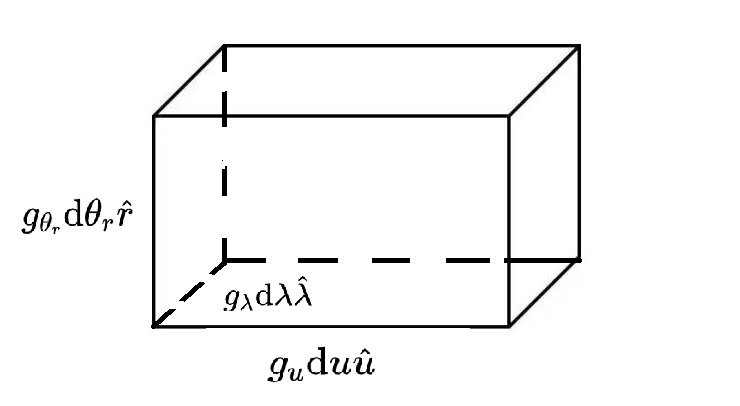
\includegraphics[width=0.7\linewidth]{rectangle.jpg}
	\caption{$\mathrm{d}\vec{r}$三个分量构成的平行六面体}
	\label{fig:1}
\end{figure}
则由高斯定理
\[
\div \vec{A} \; g_u g_{\theta_r}g_\lambda \mathrm{d}u \mathrm{d}\theta_r \mathrm{d}\lambda = \oint_S \vec{A}\cdot \mathrm{d}\vec{S}\eqno(2)
\]
右式表示对整个平行六面体的六个面作通量积分。先考察前后两个面的通量
\[
\vec{A}\cdot \mathrm{d}\vec{S}_{\text{前后}} = - A_\lambda g_u g_{\theta_r}\mathrm{d}u \mathrm{d}\theta_r {\Bigg|}_\lambda + A_\lambda g_u g_{\theta_r}\mathrm{d}u \mathrm{d}\theta_r {\Bigg|}_{\lambda + \mathrm{d}\lambda} = \frac{\partial}{\partial \lambda} (A_\lambda g_u g_{\theta_r})\mathrm{d}u \mathrm{d}\theta_r \mathrm{d}\lambda
\]
类似可以得到左右、上下两个面的通量,于是
\[
 \oint_S \vec{A}\cdot \mathrm{d}\vec{S} = \left[\frac{\partial}{\partial \lambda} (A_\lambda g_u g_{\theta_r}) + \frac{\partial}{\partial \theta_r} (A_{\theta_r} g_u g_{\lambda}) + \frac{\partial}{\partial u} (A_u g_{\theta_r} g_{\lambda})\right]\mathrm{d}u \mathrm{d}\theta_r \mathrm{d}\lambda
\]
代入(2)得到散度得表达式
\[
\div \vec{A} = \frac{1}{g_u g_{\theta_r} g_\lambda}\left[\frac{\partial}{\partial u} (A_u g_{\theta_r} g_{\lambda}) + \frac{\partial}{\partial \theta_r} (A_{\theta_r} g_u g_{\lambda}) + \frac{\partial}{\partial \lambda} (A_\lambda g_u g_{\theta_r}) \right]\eqno(3)
\]

最后,结合(1)(3)两式,
\[
\grad^2 f = \div \grad f = \frac{1}{g_u g_{\theta_r} g_\lambda}\left[\frac{\partial}{\partial u} (\frac{g_{\theta_r} g_{\lambda}}{g_{u}}\frac{\partial f}{\partial u}) + \frac{\partial}{\partial \theta_r} (\frac{g_u g_{\lambda}}{g_{\theta_r}}\frac{\partial f}{\partial \theta_r}) + \frac{\partial}{\partial \lambda} (\frac{g_u g_{\theta_r}}{g_\lambda}\frac{\partial f}{\partial \lambda}) \right]
\]
代入$g_u,\;g_{\theta_r},\;g_\lambda$的表达式得
\newcommand{\gu}{\dfrac{\sqrt{u^2 + E^2\cos^2\theta_r}}{\sqrt{u^2+E^2}}}
\newcommand{\gthetar}{\sqrt{u^2 + E^2\cos^2\theta_r}}
\newcommand{\glambda}{\sqrt{u^2+E^2}\sin\theta_r}

\begin{align*}
\grad^2 f & =  \dfrac{1}{\gu \gthetar \glambda}\Bigg[\dfrac{\partial}{\partial u} (\dfrac{\gthetar \glambda}{\gu}\dfrac{\partial f}{\partial u}) + \\ & \quad \dfrac{\partial}{\partial \theta_r} (\dfrac{\gu \glambda}{\gthetar}\dfrac{\partial f}{\partial \theta_r}) + \dfrac{\partial}{\partial \lambda}  (\dfrac{\gu\gthetar}{\glambda}\dfrac{\partial f}{\partial \lambda}) \Bigg]\\
& = \frac{1}{u^2+E^2\cos^2\theta_r}\Bigg[\dfrac{\partial}{\partial u}(u^2+E^2) \dfrac{\partial f}{\partial u} + \frac{1}{\sin \theta_r}\dfrac{\partial}{\partial \theta_r}(\sin \theta_r \dfrac{\partial f}{\partial \theta_r}) + \dfrac{u^2 + E^2 \cos^2 \theta_r }{(u^2+E^2\sin^2)\theta_r} \dfrac{\partial^2 f}{\partial \lambda^2}\Bigg]\\
& = \frac{1}{u^2+E^2\cos^2\theta_r}\Bigg[\dfrac{\partial}{\partial u}(u^2+E^2) \dfrac{\partial}{\partial u} + \frac{1}{\sin \theta_r}\dfrac{\partial}{\partial \theta_r}(\sin \theta_r \dfrac{\partial}{\partial \theta_r}) + \dfrac{u^2 + E^2 \cos^2 \theta_r }{(u^2+E^2\sin^2)\theta_r} \dfrac{\partial^2}{\partial \lambda^2}\Bigg] f
\end{align*}
从而椭球坐标系中拉普拉斯算符的表达式为
\[
\grad^2 = \frac{1}{u^2+E^2\cos^2\theta_r}\Bigg[\dfrac{\partial}{\partial u}(u^2+E^2 \dfrac{\partial}{\partial u}) + \frac{1}{\sin \theta_r}\dfrac{\partial}{\partial \theta_r}(\sin \theta_r \dfrac{\partial}{\partial \theta_r}) + \dfrac{u^2 + E^2 \cos^2 \theta_r }{(u^2+E^2\sin^2)\theta_r} \dfrac{\partial^2}{\partial \lambda^2}\Bigg]
\]

\end{document}